%template1.tex
%The following LaTeX source file represents the simplest kind of slide presentation; no overlays, no included graphics. Substitute your favorite style for ``pascal''. To create the PDF file template1.pdf, (1) be sure to use the prosper class, then (2) execute the command latex template1.tex, and (3) the command dvipdf template1.dvi.

%%%%%%%%%%%%%%%%%%%%%%%%%%%%%%% template1.tex %%%%%%%%%%%%%%%%%%%%%%%%%%%%%%%%%%%
\documentclass[a4paper,blends,pdf,colorBG,slideColor]{prosper}
% definitions for slides for CSC544
% Lutz Hamel, (c) 2007

\hypersetup{pdfpagemode=FullScreen}

\usepackage{times}
\usepackage{latexsym}
\usepackage{alltt}
\usepackage{booktabs}
\usepackage{amsmath}
\usepackage{amsopn}
\usepackage{amsfonts}
\usepackage{amssymb}
%\usepackage[usenames]{color}

\def\sign{\qopname\relax{no}{sign}}
\def\argmax{\qopname\relax{no}{argmax}}
\def\argmin{\qopname\relax{no}{argmin}}

\newcommand{\grad}{\ensuremath{\nabla}} 
\newcommand{\loss}{\ensuremath{{\cal L}}}
\newcommand{\err}{\mbox{err}}
\newcommand{\mse}{\mbox{mse}}
\newcommand{\acc}{\mbox{acc}}
\newcommand{\Integer}{\ensuremath{\mathbb{N}}}
\newcommand{\size}[1]{{|{#1}|}}
\newcommand{\Rnspace}[1]{\ensuremath{\mathbb{R}^{#1}}}
\newcommand{\Real}{\ensuremath{\mathbb{R}}}
\newcommand{\mytt}[1]{{\small\tt{#1}}}
\newcommand{\textemph}[1]{{\em #1}}
\newcommand{\suchthat}{\mid}
\newcommand{\orbar}{\;|\;}
\newcommand{\bs}[1]{\begin{slide}{#1}\ptsize{8}}
\newcommand{\es}{\end{slide}}
\newcommand{\co}{\,\colon\;}
\newcommand{\pair}[2]{\ensuremath{( {#1}, {#2} )}}
\newcommand{\model}[1]{\hat{#1}}
\newcommand{\ul}[1]{{\bf\em #1}}
\newcommand{\ol}{\overline}
\newcommand{\definition}[1]{{\bf Definition: }{\em #1}}
\newcommand{\example}[1]{{\bf Example: }{#1}}
\newcommand{\abs}[1]{|{#1}|}
\newcommand{\mytab}{\makebox[.1in]{}}

\newcommand{\fdef}[1]{
\begin{center}
\fbox{
\begin{minipage}{3.5in}
{\bf Definition:}
{#1}
\end{minipage}
}
\end{center}
}

\newcommand{\fframe}[1]{
\begin{center}
\fbox{
\begin{minipage}{3.5in}
{#1}
\end{minipage}
}
\end{center}
}

\newcommand{\nframe}[1]{
\begin{center}
\begin{minipage}{3.5in}
{#1}
\end{minipage}
\end{center}
}

\newenvironment{Rcode}
	{
		\scriptsize
		\begin{quote}
		\begin{alltt}
	}
	{
		\end{alltt}
		\end{quote}
	}




\begin{document}

\bs{Confidence Intervals}
\vspace{.2in}
{\bf Observation:} It does not matter how careful we are with our model evaluation techniques,
there remains a fundamental uncertainty about the ability of our data set $D$ to effectively
represent our (possibly infinite) data universe.

This uncertainty reflects into our model evaluation.  If $D$ is a poor representation then
the models we construct using $D$ will generalize poorly to the rest of the data universe.  If
$D$ is a good representation of the data universe then we can expect that our model will
generalize well.

Here we will deal with this uncertainty using {\em confidence intervals}.

Perhaps most surprising is that we will use $D$ itself in order to estimate this uncertainty using
the {\em bootstrap}.
\es

\bs{Confidence Intervals}
First, let us define {\em error confidence intervals} formally.

Given a model error $\err_D$ over some data set $D$,  then
the error confidence interval is defined as  the probability $p$ that our model error $\err_D$ lies between some lower bound $\text{lb}$ and some upper bound $\text{ub}$,
\begin{equation*}
Pr\left(\text{lb} \le \err_D \le \text{ub}\right) = p.
\end{equation*}
Paraphrasing this equation with $p=95\%$: 
\begin{center}
\fframe{\em We are $95\%$ percent sure
 that our error $\err_D$ is not better than $\text{lb}$ and not worse than $\text{ub}$.}
\end{center}
\es

\bs{The Bootstrap}
\small
A particular effective and computationally straightforward way to estimate the lower and upper bounds of confidence intervals is the {\em bootstrap}.  

What is remarkable about the bootstrap is that we use the data set $D$ itself to capture the uncertainty
with which it represents the data universe at large.

In the bootstrap we create $b$ bootstrap samples of our data set $D$  using sampling with replacement.

We use the variation among the bootstrap samples to compute the variation in the respective model errors.

\vspace{.2in}
\begin{center}
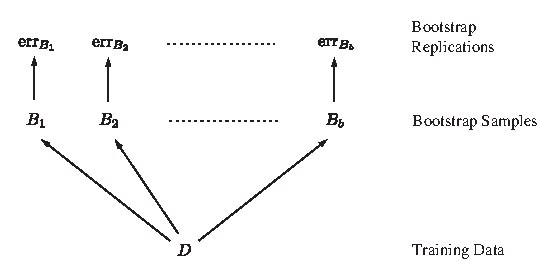
\includegraphics[height=30mm]{figures/fig09-03.eps}
\end{center}
\es

\bs{The Bootstrap}
\vspace{.2in}
\fframe{
{\rm given data set $D$}\\
{\bf for} $i = 1$ {\bf to} $200$ {\bf do}\\
\mytab $B[i]\leftarrow$ {\rm sample $D$ with replacement, note $\size{B[i]} = \size{D}$.}\\
\mytab $\err[i] \leftarrow$ {\rm compute model error using parameter set $(k^*,\lambda^*,C^*)$ and $B[i]$.}\\
{\bf end for}\\
{\rm sort $\err$ in ascending fashion}\\
$\text{ub} \leftarrow \err[195]$\\
$\text{lb} \leftarrow \err[5]$\\
{\bf return} $(\text{lb},\text{ub})$
}
\begin{center}
The algorithm to compute a $95\%$ error confidence interval.
\end{center}
\es

\bs{Model Comparisons}
By now it should be clear that a single performance number computed on $D$ is perhaps a poor
indicator for models.

As an example, consider the model $\model{f}_D[k^*,\lambda^*,C^*]$ with a cross-validated error,
\begin{equation*}
\text{CVE}_D[k^*,\lambda^*,C^*] = 0.1,
\end{equation*}
and a $95\%$ confidence interval ${\color{red}[0.08,0.12]}$.
Consider another model $\model{f}_D[k^\bullet,\lambda^\bullet,C^\bullet]$ with a cross-validated error,
\begin{equation*}
\text{CVE}_D[k^\bullet,\lambda^\bullet,C^\bullet] = 0.05,
\end{equation*}
and a $95\%$ confidence interval ${\color{red}[0.01,0.09]}$.  

By just looking at the cross-validated error we are tempted to say that the second model is
superior to the first model.

However, the confidence intervals {\em overlap}, meaning that the performance difference between
the two models is {\em statistically not significant}.
\es

\end{document}
%%%%%%%%%%%%%%%%%%%%%%%%%%% end of template1.tex %%%%%%%%%%%%%%%%%%%%%%%%%%%%%%%%

